\documentclass[twoside]{book}

% Packages required by doxygen
\usepackage{calc}
\usepackage{doxygen}
\usepackage{graphicx}
\usepackage[utf8]{inputenc}
\usepackage{makeidx}
\usepackage{multicol}
\usepackage{multirow}
\usepackage{textcomp}
\usepackage[table]{xcolor}

% Font selection
\usepackage[T1]{fontenc}
\usepackage{mathptmx}
\usepackage[scaled=.90]{helvet}
\usepackage{courier}
\usepackage{amssymb}
\usepackage{sectsty}
\renewcommand{\familydefault}{\sfdefault}
\allsectionsfont{%
  \fontseries{bc}\selectfont%
  \color{darkgray}%
}
\renewcommand{\DoxyLabelFont}{%
  \fontseries{bc}\selectfont%
  \color{darkgray}%
}

% Page & text layout
\usepackage{geometry}
\geometry{%
  a4paper,%
  top=2.5cm,%
  bottom=2.5cm,%
  left=2.5cm,%
  right=2.5cm%
}
\tolerance=750
\hfuzz=15pt
\hbadness=750
\setlength{\emergencystretch}{15pt}
\setlength{\parindent}{0cm}
\setlength{\parskip}{0.2cm}
\makeatletter
\renewcommand{\paragraph}{%
  \@startsection{paragraph}{4}{0ex}{-1.0ex}{1.0ex}{%
    \normalfont\normalsize\bfseries\SS@parafont%
  }%
}
\renewcommand{\subparagraph}{%
  \@startsection{subparagraph}{5}{0ex}{-1.0ex}{1.0ex}{%
    \normalfont\normalsize\bfseries\SS@subparafont%
  }%
}
\makeatother

% Headers & footers
\usepackage{fancyhdr}
\pagestyle{fancyplain}
\fancyhead[LE]{\fancyplain{}{\bfseries\thepage}}
\fancyhead[CE]{\fancyplain{}{}}
\fancyhead[RE]{\fancyplain{}{\bfseries\leftmark}}
\fancyhead[LO]{\fancyplain{}{\bfseries\rightmark}}
\fancyhead[CO]{\fancyplain{}{}}
\fancyhead[RO]{\fancyplain{}{\bfseries\thepage}}
\fancyfoot[LE]{\fancyplain{}{}}
\fancyfoot[CE]{\fancyplain{}{}}
\fancyfoot[RE]{\fancyplain{}{\bfseries\scriptsize Generated on Wed Sep 12 2018 11\-:31\-:12 for cjr by Doxygen }}
\fancyfoot[LO]{\fancyplain{}{\bfseries\scriptsize Generated on Wed Sep 12 2018 11\-:31\-:12 for cjr by Doxygen }}
\fancyfoot[CO]{\fancyplain{}{}}
\fancyfoot[RO]{\fancyplain{}{}}
\renewcommand{\footrulewidth}{0.4pt}
\renewcommand{\chaptermark}[1]{%
  \markboth{#1}{}%
}
\renewcommand{\sectionmark}[1]{%
  \markright{\thesection\ #1}%
}

% Indices & bibliography
\usepackage{natbib}
\usepackage[titles]{tocloft}
\setcounter{tocdepth}{3}
\setcounter{secnumdepth}{5}
\makeindex

% Hyperlinks (required, but should be loaded last)
\usepackage{ifpdf}
\ifpdf
  \usepackage[pdftex,pagebackref=true]{hyperref}
\else
  \usepackage[ps2pdf,pagebackref=true]{hyperref}
\fi
\hypersetup{%
  colorlinks=true,%
  linkcolor=blue,%
  citecolor=blue,%
  unicode%
}

% Custom commands
\newcommand{\clearemptydoublepage}{%
  \newpage{\pagestyle{empty}\cleardoublepage}%
}


%===== C O N T E N T S =====

\begin{document}

% Titlepage & ToC
\hypersetup{pageanchor=false}
\pagenumbering{roman}
\begin{titlepage}
\vspace*{7cm}
\begin{center}%
{\Large cjr }\\
\vspace*{1cm}
{\large Generated by Doxygen 1.8.5}\\
\vspace*{0.5cm}
{\small Wed Sep 12 2018 11:31:12}\\
\end{center}
\end{titlepage}
\clearemptydoublepage
\tableofcontents
\clearemptydoublepage
\pagenumbering{arabic}
\hypersetup{pageanchor=true}

%--- Begin generated contents ---
\chapter{Bug List}
\label{bug}
\hypertarget{bug}{}

\begin{DoxyRefList}
\item[\label{bug__bug000001}%
\hypertarget{bug__bug000001}{}%
Group \hyperlink{classcjr_1_1number_amgrpf308c32226026625205207ec76528501}{Universal Values} ]Undefined behaviour when making calculations only on these values. 
\end{DoxyRefList}
\chapter{Hierarchical Index}
\section{Class Hierarchy}
This inheritance list is sorted roughly, but not completely, alphabetically\-:\begin{DoxyCompactList}
\item \contentsline{section}{cjr\-:\-:base\-Range}{\pageref{classcjr_1_1base_range}}{}
\item exception\begin{DoxyCompactList}
\item \contentsline{section}{cjr\-:\-:exception\-:\-:exception}{\pageref{classcjr_1_1exception_1_1exception}}{}
\begin{DoxyCompactList}
\item \contentsline{section}{cjr\-:\-:exception\-:\-:different\-Base\-Exception}{\pageref{classcjr_1_1exception_1_1different_base_exception}}{}
\item \contentsline{section}{cjr\-:\-:exception\-:\-:invalid\-Base\-Exception}{\pageref{classcjr_1_1exception_1_1invalid_base_exception}}{}
\end{DoxyCompactList}
\end{DoxyCompactList}
\item \contentsline{section}{cjr\-:\-:number$<$ B $>$}{\pageref{classcjr_1_1number}}{}
\end{DoxyCompactList}

\chapter{Class Index}
\section{Class List}
Here are the classes, structs, unions and interfaces with brief descriptions\-:\begin{DoxyCompactList}
\item\contentsline{section}{\hyperlink{classcjr_1_1base_range}{cjr\-::base\-Range} \\*Class defining ranges of bases for \hyperlink{classcjr_1_1number}{number} }{\pageref{classcjr_1_1base_range}}{}
\item\contentsline{section}{\hyperlink{classcjr_1_1exception_1_1different_base_exception}{cjr\-::exception\-::different\-Base\-Exception} \\*Exception to be thrown when two numbers have different bases }{\pageref{classcjr_1_1exception_1_1different_base_exception}}{}
\item\contentsline{section}{\hyperlink{classcjr_1_1exception_1_1division_by_zero_exception}{cjr\-::exception\-::division\-By\-Zero\-Exception} \\*Exception to be thrown when division by 0 occurs }{\pageref{classcjr_1_1exception_1_1division_by_zero_exception}}{}
\item\contentsline{section}{\hyperlink{classcjr_1_1exception_1_1exception}{cjr\-::exception\-::exception} \\*Universal exception for cjr }{\pageref{classcjr_1_1exception_1_1exception}}{}
\item\contentsline{section}{\hyperlink{classcjr_1_1exception_1_1invalid_base_exception}{cjr\-::exception\-::invalid\-Base\-Exception} \\*Exception to be thrown when given base is invalid }{\pageref{classcjr_1_1exception_1_1invalid_base_exception}}{}
\item\contentsline{section}{\hyperlink{classcjr_1_1number}{cjr\-::number$<$ B $>$} \\*Class for storing numbers of any size }{\pageref{classcjr_1_1number}}{}
\end{DoxyCompactList}

\chapter{File Index}
\section{File List}
Here is a list of all documented files with brief descriptions\-:\begin{DoxyCompactList}
\item\contentsline{section}{src/\hyperlink{cjr_8hpp}{cjr.\-hpp} \\*Includes all of std headers and external libraries needed by the project }{\pageref{cjr_8hpp}}{}
\item\contentsline{section}{src/exceptions/{\bfseries exception.\-hpp} }{\pageref{exception_8hpp}}{}
\item\contentsline{section}{src/exceptions/\hyperlink{number_exceptions_8hpp}{number\-Exceptions.\-hpp} \\*Contains custom exceptions for number }{\pageref{number_exceptions_8hpp}}{}
\item\contentsline{section}{src/numbers/{\bfseries number.\-hpp} }{\pageref{number_8hpp}}{}
\item\contentsline{section}{src/numbers/{\bfseries utils.\-hpp} }{\pageref{utils_8hpp}}{}
\end{DoxyCompactList}

\chapter{Class Documentation}
\hypertarget{classcjr_1_1base_range}{\section{cjr\-:\-:base\-Range Class Reference}
\label{classcjr_1_1base_range}\index{cjr\-::base\-Range@{cjr\-::base\-Range}}
}


\subsection{Detailed Description}
a class defining ranges of bases for \hyperlink{classcjr_1_1number}{number} 

It is used as a template parameter for \hyperlink{classcjr_1_1number}{number}. The maximal values of bases are calculated inside \hyperlink{classcjr_1_1number}{number}. 

{\ttfamily \#include $<$utils.\-hpp$>$}

\subsection*{Public Types}
\begin{DoxyCompactItemize}
\item 
using \hyperlink{classcjr_1_1base_range_a5f25722f51adfdcb6568431af1ac3cfb}{binary} = bool
\item 
\hypertarget{classcjr_1_1base_range_a2b08ecad9edd4a2dce0a9dc376d2fbd5}{using {\bfseries small} = short int}\label{classcjr_1_1base_range_a2b08ecad9edd4a2dce0a9dc376d2fbd5}

\item 
\hypertarget{classcjr_1_1base_range_aae4aa19dc5ab582bf196cbf913c743ca}{using {\bfseries medium} = int}\label{classcjr_1_1base_range_aae4aa19dc5ab582bf196cbf913c743ca}

\item 
\hypertarget{classcjr_1_1base_range_ad572b09254a0b5d48559271eceb420ff}{using {\bfseries big} = long int}\label{classcjr_1_1base_range_ad572b09254a0b5d48559271eceb420ff}

\item 
\hypertarget{classcjr_1_1base_range_a9ba9a270901aedd4344df7bd748ee03c}{using {\bfseries huge} = long long int}\label{classcjr_1_1base_range_a9ba9a270901aedd4344df7bd748ee03c}

\end{DoxyCompactItemize}
\subsection*{Static Public Member Functions}
\begin{DoxyCompactItemize}
\item 
\hypertarget{classcjr_1_1base_range_a353bdf3cc3ffade6dd4cac9c1cac7268}{{\footnotesize template$<$class B $>$ }\\static const std\-::string {\bfseries get\-Range\-Name} (const B \&given\-Base, const bool \&extended=false)}\label{classcjr_1_1base_range_a353bdf3cc3ffade6dd4cac9c1cac7268}

\end{DoxyCompactItemize}


\subsection{Member Typedef Documentation}
\hypertarget{classcjr_1_1base_range_a5f25722f51adfdcb6568431af1ac3cfb}{\index{cjr\-::base\-Range@{cjr\-::base\-Range}!binary@{binary}}
\index{binary@{binary}!cjr::baseRange@{cjr\-::base\-Range}}
\subsubsection[{binary}]{\setlength{\rightskip}{0pt plus 5cm}using {\bf cjr\-::base\-Range\-::binary} =  bool}}\label{classcjr_1_1base_range_a5f25722f51adfdcb6568431af1ac3cfb}
\begin{DoxyWarning}{Warning}
N\-O\-T Y\-E\-T I\-M\-P\-L\-E\-M\-E\-N\-T\-E\-D
\end{DoxyWarning}
\hyperlink{classcjr_1_1base_range}{base\-Range} for storing binary numbers 

The documentation for this class was generated from the following file\-:\begin{DoxyCompactItemize}
\item 
src/numbers/utils.\-hpp\end{DoxyCompactItemize}

\hypertarget{classcjr_1_1exception_1_1different_base_exception}{\section{cjr\-:\-:exception\-:\-:different\-Base\-Exception Class Reference}
\label{classcjr_1_1exception_1_1different_base_exception}\index{cjr\-::exception\-::different\-Base\-Exception@{cjr\-::exception\-::different\-Base\-Exception}}
}


\subsection{Detailed Description}
Exception to be thrown when two numbers have different bases. 

{\ttfamily \#include $<$number\-Exceptions.\-hpp$>$}

Inheritance diagram for cjr\-:\-:exception\-:\-:different\-Base\-Exception\-:\begin{figure}[H]
\begin{center}
\leavevmode
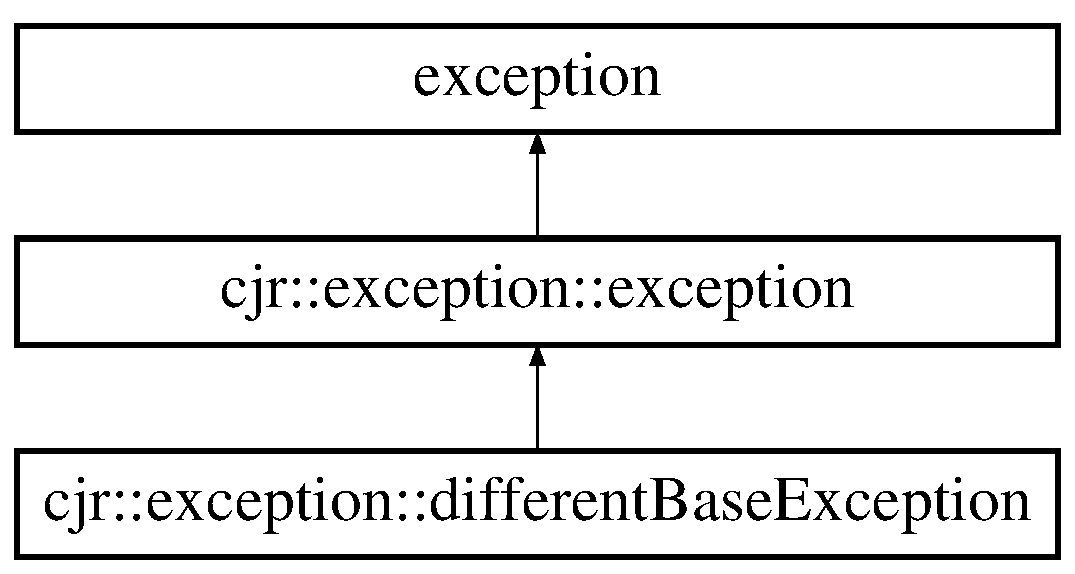
\includegraphics[height=3.000000cm]{classcjr_1_1exception_1_1different_base_exception}
\end{center}
\end{figure}
\subsection*{Additional Inherited Members}


The documentation for this class was generated from the following file\-:\begin{DoxyCompactItemize}
\item 
src/exceptions/\hyperlink{number_exceptions_8hpp}{number\-Exceptions.\-hpp}\end{DoxyCompactItemize}

\hypertarget{classcjr_1_1exception_1_1division_by_zero_exception}{\section{cjr\-:\-:exception\-:\-:division\-By\-Zero\-Exception Class Reference}
\label{classcjr_1_1exception_1_1division_by_zero_exception}\index{cjr\-::exception\-::division\-By\-Zero\-Exception@{cjr\-::exception\-::division\-By\-Zero\-Exception}}
}


\subsection{Detailed Description}
Exception to be thrown when division by 0 occurs. 

{\ttfamily \#include $<$number\-Exceptions.\-hpp$>$}

Inheritance diagram for cjr\-:\-:exception\-:\-:division\-By\-Zero\-Exception\-:\begin{figure}[H]
\begin{center}
\leavevmode
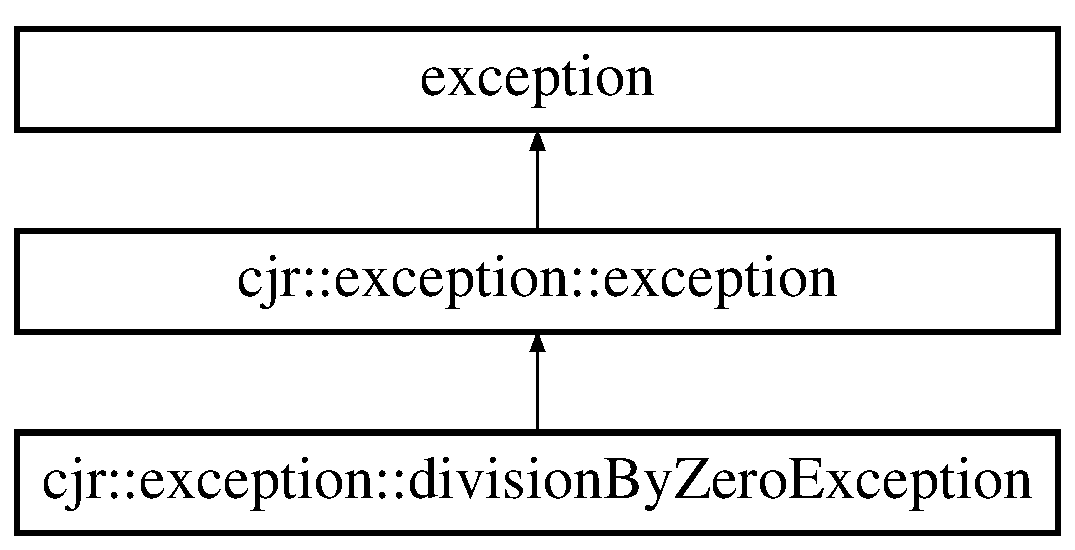
\includegraphics[height=3.000000cm]{classcjr_1_1exception_1_1division_by_zero_exception}
\end{center}
\end{figure}
\subsection*{Additional Inherited Members}


The documentation for this class was generated from the following file\-:\begin{DoxyCompactItemize}
\item 
src/exceptions/\hyperlink{number_exceptions_8hpp}{number\-Exceptions.\-hpp}\end{DoxyCompactItemize}

\hypertarget{classcjr_1_1exception_1_1exception}{\section{cjr\-:\-:exception\-:\-:exception Class Reference}
\label{classcjr_1_1exception_1_1exception}\index{cjr\-::exception\-::exception@{cjr\-::exception\-::exception}}
}


\subsection{Detailed Description}
Universal exception for cjr. 

{\ttfamily \#include $<$exception.\-hpp$>$}

Inheritance diagram for cjr\-:\-:exception\-:\-:exception\-:\begin{figure}[H]
\begin{center}
\leavevmode
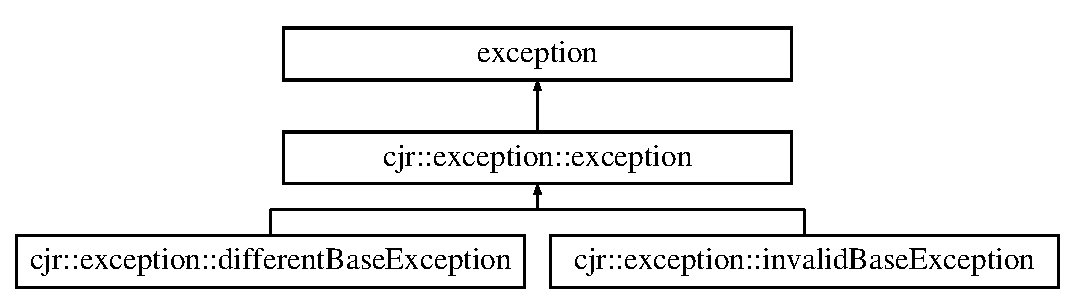
\includegraphics[height=3.000000cm]{classcjr_1_1exception_1_1exception}
\end{center}
\end{figure}
\subsection*{Public Member Functions}
\begin{DoxyCompactItemize}
\item 
\hypertarget{classcjr_1_1exception_1_1exception_a7c359250e31f93a5f9fb20d4963cd029}{{\bfseries exception} (const std\-::string \&given\-Message)}\label{classcjr_1_1exception_1_1exception_a7c359250e31f93a5f9fb20d4963cd029}

\item 
\hypertarget{classcjr_1_1exception_1_1exception_a3a06a05cdfda3d492b5fa6a21c3dd177}{const char $\ast$ {\bfseries what} () const noexceptoverride}\label{classcjr_1_1exception_1_1exception_a3a06a05cdfda3d492b5fa6a21c3dd177}

\end{DoxyCompactItemize}
\subsection*{Protected Attributes}
\begin{DoxyCompactItemize}
\item 
\hypertarget{classcjr_1_1exception_1_1exception_a9197ebb57c1aae9af36848bb2bfb1886}{char $\ast$ \hyperlink{classcjr_1_1exception_1_1exception_a9197ebb57c1aae9af36848bb2bfb1886}{message}}\label{classcjr_1_1exception_1_1exception_a9197ebb57c1aae9af36848bb2bfb1886}

\begin{DoxyCompactList}\small\item\em Message to be displayed with error. \end{DoxyCompactList}\end{DoxyCompactItemize}


The documentation for this class was generated from the following file\-:\begin{DoxyCompactItemize}
\item 
src/exceptions/exception.\-hpp\end{DoxyCompactItemize}

\hypertarget{classcjr_1_1exception_1_1invalid_base_exception}{\section{cjr\-:\-:exception\-:\-:invalid\-Base\-Exception Class Reference}
\label{classcjr_1_1exception_1_1invalid_base_exception}\index{cjr\-::exception\-::invalid\-Base\-Exception@{cjr\-::exception\-::invalid\-Base\-Exception}}
}


\subsection{Detailed Description}
Exception to be thrown when given base is invalid. 

Base is invalid when it is less or equal to zero or it exceed base maximum. 

{\ttfamily \#include $<$number\-Exceptions.\-hpp$>$}

Inheritance diagram for cjr\-:\-:exception\-:\-:invalid\-Base\-Exception\-:\begin{figure}[H]
\begin{center}
\leavevmode
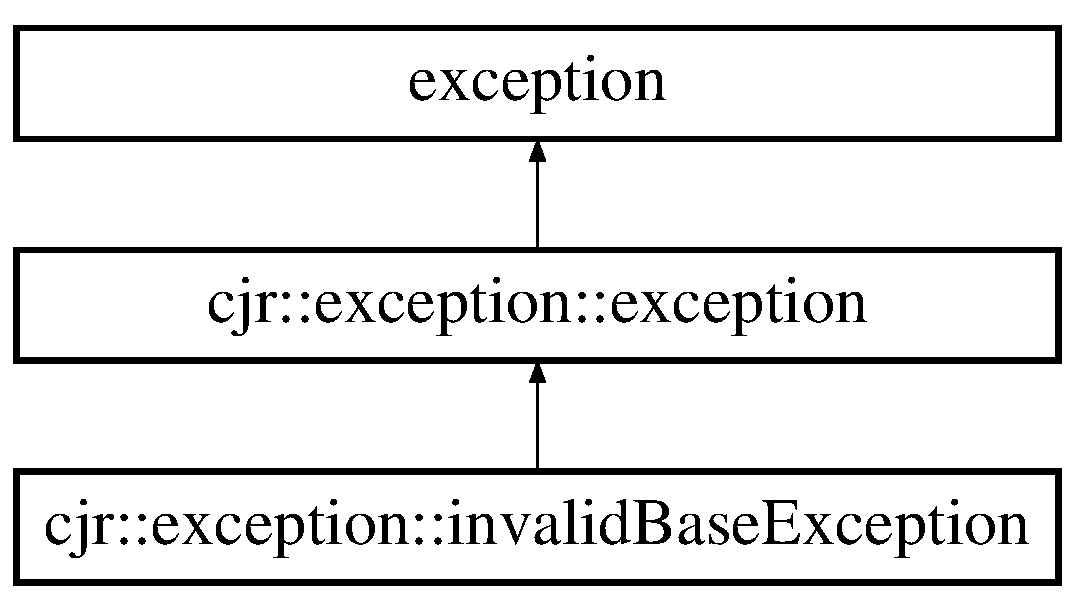
\includegraphics[height=3.000000cm]{classcjr_1_1exception_1_1invalid_base_exception}
\end{center}
\end{figure}
\subsection*{Public Member Functions}
\begin{DoxyCompactItemize}
\item 
\hypertarget{classcjr_1_1exception_1_1invalid_base_exception_a1642100156f3313b9f762a1fff75588c}{{\footnotesize template$<$class B $>$ }\\{\bfseries invalid\-Base\-Exception} (const B \&given\-Base, const B \&max\-Base)}\label{classcjr_1_1exception_1_1invalid_base_exception_a1642100156f3313b9f762a1fff75588c}

\end{DoxyCompactItemize}
\subsection*{Additional Inherited Members}


The documentation for this class was generated from the following file\-:\begin{DoxyCompactItemize}
\item 
src/exceptions/\hyperlink{number_exceptions_8hpp}{number\-Exceptions.\-hpp}\end{DoxyCompactItemize}

\hypertarget{classcjr_1_1number}{\section{cjr\-:\-:number$<$ B $>$ Class Template Reference}
\label{classcjr_1_1number}\index{cjr\-::number$<$ B $>$@{cjr\-::number$<$ B $>$}}
}


\subsection{Detailed Description}
\subsubsection*{template$<$class B = base\-Range\-::medium$>$class cjr\-::number$<$ B $>$}

a class for storing numbers of any size 


\begin{DoxyTemplParams}{Template Parameters}
{\em B} & defines maximal base of the number, see \hyperlink{classcjr_1_1base_range}{base\-Range} \\
\hline
\end{DoxyTemplParams}


{\ttfamily \#include $<$number.\-hpp$>$}

\subsection*{Public Types}
\begin{DoxyCompactItemize}
\item 
\hypertarget{classcjr_1_1number_a64ca3e7862f3f4940065b93d38c1a465}{using \hyperlink{classcjr_1_1number_a64ca3e7862f3f4940065b93d38c1a465}{digit\-List} = std\-::list$<$ B $>$}\label{classcjr_1_1number_a64ca3e7862f3f4940065b93d38c1a465}

\begin{DoxyCompactList}\small\item\em List type for storing digits of \hyperlink{classcjr_1_1number}{number}. \end{DoxyCompactList}\item 
\hypertarget{classcjr_1_1number_a137416a57d724f8b6a5c14bab7c6802b}{using \hyperlink{classcjr_1_1number_a137416a57d724f8b6a5c14bab7c6802b}{digit\-Iterator} = typename std\-::list$<$ B $>$\-::iterator}\label{classcjr_1_1number_a137416a57d724f8b6a5c14bab7c6802b}

\begin{DoxyCompactList}\small\item\em Iterator type for storing iterators for \hyperlink{classcjr_1_1number_a64ca3e7862f3f4940065b93d38c1a465}{digit\-List}. \end{DoxyCompactList}\end{DoxyCompactItemize}
\subsection*{Public Member Functions}
\begin{DoxyCompactItemize}
\item 
\hypertarget{classcjr_1_1number_a96952d8729d8a96590b5cfa4de8c94f9}{\hyperlink{classcjr_1_1number_a96952d8729d8a96590b5cfa4de8c94f9}{number} ()}\label{classcjr_1_1number_a96952d8729d8a96590b5cfa4de8c94f9}

\begin{DoxyCompactList}\small\item\em Constructs new number with 0 value and 10 as base. \end{DoxyCompactList}\item 
\hyperlink{classcjr_1_1number_aeaf08725e9ae255c3ee25045bbd235f1}{number} (const B \&init\-Value, const B \&base=10)
\begin{DoxyCompactList}\small\item\em Constructs new number with given value and base. \end{DoxyCompactList}\item 
\hyperlink{classcjr_1_1number_aa3ab519d30cba11bfec2177c2b429b8f}{number} (const \hyperlink{classcjr_1_1number}{number}$<$ B $>$ \&source\-Number)
\begin{DoxyCompactList}\small\item\em Copy constructor for \hyperlink{classcjr_1_1number}{number}. \end{DoxyCompactList}\end{DoxyCompactItemize}
\begin{Indent}{\bf Utility}\par
\begin{DoxyCompactItemize}
\item 
void \hyperlink{classcjr_1_1number_a14c7b4e829ee04a405f149db57c00195}{set\-Value} (const \hyperlink{classcjr_1_1number}{number}$<$ B $>$ \&n)
\begin{DoxyCompactList}\small\item\em sets new value of the number \end{DoxyCompactList}\item 
void \hyperlink{classcjr_1_1number_a66c1ad13348c078cbf75d73def0aab9e}{set\-Value} (const B \&new\-Value)
\begin{DoxyCompactList}\small\item\em sets new value of the number \end{DoxyCompactList}\item 
\hypertarget{classcjr_1_1number_a456c3bd567b3603b9985d6baa73f8641}{const bool \hyperlink{classcjr_1_1number_a456c3bd567b3603b9985d6baa73f8641}{is\-Zero} () const }\label{classcjr_1_1number_a456c3bd567b3603b9985d6baa73f8641}

\begin{DoxyCompactList}\small\item\em returns true when number's value is 0 \end{DoxyCompactList}\item 
\hypertarget{classcjr_1_1number_a08274244f62ed97d98464046697cb800}{const bool \& \hyperlink{classcjr_1_1number_a08274244f62ed97d98464046697cb800}{is\-Negative} () const noexcept}\label{classcjr_1_1number_a08274244f62ed97d98464046697cb800}

\begin{DoxyCompactList}\small\item\em returns true when number's value is less than 0 \end{DoxyCompactList}\item 
\hypertarget{classcjr_1_1number_a153b7f8c8223b47846e2c64c7bdccfdb}{void \hyperlink{classcjr_1_1number_a153b7f8c8223b47846e2c64c7bdccfdb}{revert\-Sign} ()}\label{classcjr_1_1number_a153b7f8c8223b47846e2c64c7bdccfdb}

\begin{DoxyCompactList}\small\item\em reverts the sign of the number \end{DoxyCompactList}\item 
\hypertarget{classcjr_1_1number_a0a5c6272d8c076e1b1884530bcedee9b}{const \hyperlink{classcjr_1_1number}{number}$<$ B $>$ \hyperlink{classcjr_1_1number_a0a5c6272d8c076e1b1884530bcedee9b}{absolute\-Value} () const }\label{classcjr_1_1number_a0a5c6272d8c076e1b1884530bcedee9b}

\begin{DoxyCompactList}\small\item\em returns absolute value of the number \end{DoxyCompactList}\item 
const std\-::string \hyperlink{classcjr_1_1number_a4eb89bde4b4866e761170d6c47dd46ab}{to\-String} (const bool \&with\-Separators=false) const 
\begin{DoxyCompactList}\small\item\em returns value of the number converted to String \end{DoxyCompactList}\item 
void \hyperlink{classcjr_1_1number_aab0fd6f29b9b3ab88fbead6aa7d4dba8}{print} (const bool \&with\-Separators=false) const 
\begin{DoxyCompactList}\small\item\em prints to the console value of to\-String(bool) with new line at the end \end{DoxyCompactList}\end{DoxyCompactItemize}
\end{Indent}
\begin{Indent}{\bf Calculation}\par
{\em \begin{DoxyNote}{Note}
Making calculations on numbers with different bases gives different\-Base\-Exception 

When a std value is added to the \hyperlink{classcjr_1_1number}{number} it assumes, that the std value is represented in decimal system. Nevertheless you can add it to the \hyperlink{classcjr_1_1number}{number} of any base. 
\end{DoxyNote}
}\begin{DoxyCompactItemize}
\item 
\hypertarget{classcjr_1_1number_a314f5ddd4ea8b6e0ff752d9ca8f00a2a}{void \hyperlink{classcjr_1_1number_a314f5ddd4ea8b6e0ff752d9ca8f00a2a}{increment} ()}\label{classcjr_1_1number_a314f5ddd4ea8b6e0ff752d9ca8f00a2a}

\begin{DoxyCompactList}\small\item\em Increments the number. \end{DoxyCompactList}\item 
\hypertarget{classcjr_1_1number_af50a7633da47b4003ae722138717ecce}{void \hyperlink{classcjr_1_1number_af50a7633da47b4003ae722138717ecce}{operator++} ()}\label{classcjr_1_1number_af50a7633da47b4003ae722138717ecce}

\begin{DoxyCompactList}\small\item\em Pre-\/increments the number. \end{DoxyCompactList}\item 
\hypertarget{classcjr_1_1number_a6b6ef41013a16ea2a0cfebd5b9d99172}{const \hyperlink{classcjr_1_1number}{number}$<$ B $>$ \hyperlink{classcjr_1_1number_a6b6ef41013a16ea2a0cfebd5b9d99172}{operator++} (int)}\label{classcjr_1_1number_a6b6ef41013a16ea2a0cfebd5b9d99172}

\begin{DoxyCompactList}\small\item\em Post-\/increments the number. \end{DoxyCompactList}\item 
void \hyperlink{classcjr_1_1number_ac876a5bc8916d2ddb19a1d514ac3f5c0}{add} (const \hyperlink{classcjr_1_1number}{number}$<$ B $>$ \&number\-To\-Add)
\begin{DoxyCompactList}\small\item\em Adds given number to the number. \end{DoxyCompactList}\item 
\hypertarget{classcjr_1_1number_a3ead20a677d3bcd872895065fcfea6f7}{\hyperlink{classcjr_1_1number}{number}$<$ B $>$ \hyperlink{classcjr_1_1number_a3ead20a677d3bcd872895065fcfea6f7}{operator+} (const \hyperlink{classcjr_1_1number}{number}$<$ B $>$ \&number\-To\-Add) const }\label{classcjr_1_1number_a3ead20a677d3bcd872895065fcfea6f7}

\begin{DoxyCompactList}\small\item\em Returns the value of adding two given numbers. \end{DoxyCompactList}\item 
void \hyperlink{classcjr_1_1number_a4a3990a55896edfa85639c57d8c3c699}{add} (const B \&value\-To\-Add)
\begin{DoxyCompactList}\small\item\em Adds given std value to the number. \end{DoxyCompactList}\item 
\hypertarget{classcjr_1_1number_af4753e77a4277f4290219e4e91763d8c}{\hyperlink{classcjr_1_1number}{number}$<$ B $>$ \hyperlink{classcjr_1_1number_af4753e77a4277f4290219e4e91763d8c}{operator+} (const B \&value\-To\-Add) const }\label{classcjr_1_1number_af4753e77a4277f4290219e4e91763d8c}

\begin{DoxyCompactList}\small\item\em Returns the value of adding given number and std value. \end{DoxyCompactList}\item 
\hypertarget{classcjr_1_1number_a26eef97a8cbcf837b65e7dda206e623d}{void \hyperlink{classcjr_1_1number_a26eef97a8cbcf837b65e7dda206e623d}{decrement} ()}\label{classcjr_1_1number_a26eef97a8cbcf837b65e7dda206e623d}

\begin{DoxyCompactList}\small\item\em Decrements the number. \end{DoxyCompactList}\item 
\hypertarget{classcjr_1_1number_a2ffbd3e053d87dd7d53381df55111a79}{void \hyperlink{classcjr_1_1number_a2ffbd3e053d87dd7d53381df55111a79}{operator-\/-\/} ()}\label{classcjr_1_1number_a2ffbd3e053d87dd7d53381df55111a79}

\begin{DoxyCompactList}\small\item\em Pre-\/decrements the number. \end{DoxyCompactList}\item 
\hypertarget{classcjr_1_1number_a53449243aa05abff7e091030de0e3028}{const \hyperlink{classcjr_1_1number}{number}$<$ B $>$ \hyperlink{classcjr_1_1number_a53449243aa05abff7e091030de0e3028}{operator-\/-\/} (int)}\label{classcjr_1_1number_a53449243aa05abff7e091030de0e3028}

\begin{DoxyCompactList}\small\item\em Post-\/decrements the number. \end{DoxyCompactList}\item 
void \hyperlink{classcjr_1_1number_aa29378479836924b1110f40570198ada}{subtract} (const \hyperlink{classcjr_1_1number}{number}$<$ B $>$ \&number\-To\-Subtract)
\begin{DoxyCompactList}\small\item\em Subtracts given number from the number. \end{DoxyCompactList}\item 
\hypertarget{classcjr_1_1number_a9b54e89597d8db867a7d30bab2c8d10a}{\hyperlink{classcjr_1_1number}{number}$<$ B $>$ \hyperlink{classcjr_1_1number_a9b54e89597d8db867a7d30bab2c8d10a}{operator-\/} (const \hyperlink{classcjr_1_1number}{number}$<$ B $>$ \&number\-To\-Subtract) const }\label{classcjr_1_1number_a9b54e89597d8db867a7d30bab2c8d10a}

\begin{DoxyCompactList}\small\item\em Returns the value of subtracting two given numbers. \end{DoxyCompactList}\item 
void \hyperlink{classcjr_1_1number_af95e527ca950399a3af5dbf12d01afc5}{subtract} (const B \&value\-To\-Subtract)
\begin{DoxyCompactList}\small\item\em Subtracts given std value from the number. \end{DoxyCompactList}\item 
\hypertarget{classcjr_1_1number_ad48de2316e1e5c962c84eb4f4ad5cfc8}{\hyperlink{classcjr_1_1number}{number}$<$ B $>$ \hyperlink{classcjr_1_1number_ad48de2316e1e5c962c84eb4f4ad5cfc8}{operator-\/} (const B \&value\-To\-Subtract) const }\label{classcjr_1_1number_ad48de2316e1e5c962c84eb4f4ad5cfc8}

\begin{DoxyCompactList}\small\item\em Returns the value of subtracting std value from given number. \end{DoxyCompactList}\item 
void \hyperlink{classcjr_1_1number_a9bfb2e6eb2297527aa34f21c84c92c1c}{multiply} (const \hyperlink{classcjr_1_1number}{number}$<$ B $>$ \&number\-To\-Multiply)
\begin{DoxyCompactList}\small\item\em Multiplies the number by given \hyperlink{classcjr_1_1number}{number}. \end{DoxyCompactList}\item 
\hypertarget{classcjr_1_1number_add3f6150a03f6f1d78df5bf73eb36759}{\hyperlink{classcjr_1_1number}{number}$<$ B $>$ \hyperlink{classcjr_1_1number_add3f6150a03f6f1d78df5bf73eb36759}{operator$\ast$} (const \hyperlink{classcjr_1_1number}{number}$<$ B $>$ \&number\-To\-Multiply) const }\label{classcjr_1_1number_add3f6150a03f6f1d78df5bf73eb36759}

\begin{DoxyCompactList}\small\item\em Returns the value of multiplying the number by given \hyperlink{classcjr_1_1number}{number}. \end{DoxyCompactList}\item 
void \hyperlink{classcjr_1_1number_aea945b8aecaad22c99b954bea3af1179}{multiply} (const B \&value\-To\-Multiply)
\begin{DoxyCompactList}\small\item\em Multiplies the number by given std value. \end{DoxyCompactList}\item 
\hypertarget{classcjr_1_1number_a91b1566c18c748235fd384ed7a45f404}{\hyperlink{classcjr_1_1number}{number}$<$ B $>$ \hyperlink{classcjr_1_1number_a91b1566c18c748235fd384ed7a45f404}{operator$\ast$} (const B \&value\-To\-Multiply) const }\label{classcjr_1_1number_a91b1566c18c748235fd384ed7a45f404}

\begin{DoxyCompactList}\small\item\em Returns the value of multiplying the number by given std value. \end{DoxyCompactList}\item 
void \hyperlink{classcjr_1_1number_ace65049054fa8b2a7498a3f2af7b7298}{power} (unsigned int power=2)
\begin{DoxyCompactList}\small\item\em Raises the number to the given power. \end{DoxyCompactList}\item 
void \hyperlink{classcjr_1_1number_a5854c154e869c908da1a978698704bf3}{multiply\-By\-Base} (unsigned int \hyperlink{classcjr_1_1number_ace65049054fa8b2a7498a3f2af7b7298}{power}=1)
\begin{DoxyCompactList}\small\item\em Multiplies the number by given power of its base. \end{DoxyCompactList}\item 
void \hyperlink{classcjr_1_1number_adbcfae18aafd8466f34599c85336b27b}{divide} (\hyperlink{classcjr_1_1number}{number}$<$ B $>$ divisor)
\begin{DoxyCompactList}\small\item\em Divides the number by given \hyperlink{classcjr_1_1number}{number}. \end{DoxyCompactList}\item 
\hypertarget{classcjr_1_1number_a20e0c77b3e6467be9d6dbea40e4bfd2f}{\hyperlink{classcjr_1_1number}{number}$<$ B $>$ \hyperlink{classcjr_1_1number_a20e0c77b3e6467be9d6dbea40e4bfd2f}{operator/} (const \hyperlink{classcjr_1_1number}{number}$<$ B $>$ \&divisor) const }\label{classcjr_1_1number_a20e0c77b3e6467be9d6dbea40e4bfd2f}

\begin{DoxyCompactList}\small\item\em Returns the result of dividing the number by given \hyperlink{classcjr_1_1number}{number}. \end{DoxyCompactList}\item 
void \hyperlink{classcjr_1_1number_ae5647dac42c1e31d6c9a906be9e5a0a6}{divide} (const B \&divisor)
\begin{DoxyCompactList}\small\item\em Divides the number by given std value. \end{DoxyCompactList}\item 
\hypertarget{classcjr_1_1number_a77b8020d0a42ef040b68e31e37245af0}{\hyperlink{classcjr_1_1number}{number}$<$ B $>$ \hyperlink{classcjr_1_1number_a77b8020d0a42ef040b68e31e37245af0}{operator/} (const B \&divisor) const }\label{classcjr_1_1number_a77b8020d0a42ef040b68e31e37245af0}

\begin{DoxyCompactList}\small\item\em Returns the result of dividing the number by given std value. \end{DoxyCompactList}\item 
\hypertarget{classcjr_1_1number_a78f188be1582f5307dc6752a6e762887}{const \hyperlink{classcjr_1_1number}{number}$<$ B $>$ \hyperlink{classcjr_1_1number_a78f188be1582f5307dc6752a6e762887}{remainder} (\hyperlink{classcjr_1_1number}{number}$<$ B $>$ divisor) const }\label{classcjr_1_1number_a78f188be1582f5307dc6752a6e762887}

\begin{DoxyCompactList}\small\item\em Returns remainder of dividing the number by given \hyperlink{classcjr_1_1number}{number}. \end{DoxyCompactList}\item 
\hypertarget{classcjr_1_1number_a9aa6a071c98f597336cc587be7b88fda}{const \hyperlink{classcjr_1_1number}{number}$<$ B $>$ \hyperlink{classcjr_1_1number_a9aa6a071c98f597336cc587be7b88fda}{operator\%} (\hyperlink{classcjr_1_1number}{number}$<$ B $>$ divisor) const }\label{classcjr_1_1number_a9aa6a071c98f597336cc587be7b88fda}

\begin{DoxyCompactList}\small\item\em Returns remainder of dividing the number by given \hyperlink{classcjr_1_1number}{number}. \end{DoxyCompactList}\item 
const \hyperlink{classcjr_1_1number}{number}$<$ B $>$ \hyperlink{classcjr_1_1number_ad90db090de7ae9123bbeebd2e136aac9}{divide\-By\-Base} (unsigned int \hyperlink{classcjr_1_1number_ace65049054fa8b2a7498a3f2af7b7298}{power}=1)
\begin{DoxyCompactList}\small\item\em Divides the number by given power of its base. \end{DoxyCompactList}\end{DoxyCompactItemize}
\end{Indent}
\begin{Indent}{\bf Comparison}\par
{\em \begin{DoxyNote}{Note}
Comparing numbers with different bases gives different\-Base\-Exception 
\end{DoxyNote}
}\begin{DoxyCompactItemize}
\item 
\hypertarget{classcjr_1_1number_a16ba1ce1e338fce48151a39ded8b7474}{const bool {\bfseries is\-Bigger} (const \hyperlink{classcjr_1_1number}{number}$<$ B $>$ \&a, const bool \&or\-Equal=false) const }\label{classcjr_1_1number_a16ba1ce1e338fce48151a39ded8b7474}

\item 
\hypertarget{classcjr_1_1number_a1f8bdacbaf1f13628d0d05c0bc2d216a}{const bool {\bfseries operator$>$} (const \hyperlink{classcjr_1_1number}{number}$<$ B $>$ \&a) const }\label{classcjr_1_1number_a1f8bdacbaf1f13628d0d05c0bc2d216a}

\item 
\hypertarget{classcjr_1_1number_a409317d22923aec056b3278e844d1211}{const bool {\bfseries is\-Bigger\-Or\-Equal} (const \hyperlink{classcjr_1_1number}{number}$<$ B $>$ \&a) const }\label{classcjr_1_1number_a409317d22923aec056b3278e844d1211}

\item 
\hypertarget{classcjr_1_1number_a920c71c3a23745c99b5f80cb789cd028}{const bool {\bfseries operator$>$=} (const \hyperlink{classcjr_1_1number}{number}$<$ B $>$ \&a) const }\label{classcjr_1_1number_a920c71c3a23745c99b5f80cb789cd028}

\item 
\hypertarget{classcjr_1_1number_a5cf22a07813460edd061753af8089ca4}{const bool {\bfseries is\-Smaller} (const \hyperlink{classcjr_1_1number}{number}$<$ B $>$ \&a, const bool \&or\-Equal=false) const }\label{classcjr_1_1number_a5cf22a07813460edd061753af8089ca4}

\item 
\hypertarget{classcjr_1_1number_ab3595677812bf4fc5a19e3a7929a91da}{const bool {\bfseries operator$<$} (const \hyperlink{classcjr_1_1number}{number}$<$ B $>$ \&a) const }\label{classcjr_1_1number_ab3595677812bf4fc5a19e3a7929a91da}

\item 
\hypertarget{classcjr_1_1number_a5933f01885bea73d89cf31cc45e61d23}{const bool {\bfseries is\-Smaller\-Or\-Equal} (const \hyperlink{classcjr_1_1number}{number}$<$ B $>$ \&a) const }\label{classcjr_1_1number_a5933f01885bea73d89cf31cc45e61d23}

\item 
\hypertarget{classcjr_1_1number_a7bd4110bfd0fa3b74d1c8f39bc85f2a0}{const bool {\bfseries operator$<$=} (const \hyperlink{classcjr_1_1number}{number}$<$ B $>$ \&a) const }\label{classcjr_1_1number_a7bd4110bfd0fa3b74d1c8f39bc85f2a0}

\item 
\hypertarget{classcjr_1_1number_ae8f6c4c30da9add29b202ba0fdd280ba}{const bool {\bfseries is\-Equal} (const \hyperlink{classcjr_1_1number}{number}$<$ B $>$ \&n) const }\label{classcjr_1_1number_ae8f6c4c30da9add29b202ba0fdd280ba}

\item 
\hypertarget{classcjr_1_1number_a3ee573ccdf8c28f9c6dafa15572c27c9}{const bool {\bfseries operator==} (const \hyperlink{classcjr_1_1number}{number}$<$ B $>$ \&a) const }\label{classcjr_1_1number_a3ee573ccdf8c28f9c6dafa15572c27c9}

\item 
\hypertarget{classcjr_1_1number_aae51bdc811ee8199d5283ab4bbac32b6}{const bool {\bfseries operator!=} (const \hyperlink{classcjr_1_1number}{number}$<$ B $>$ \&a) const }\label{classcjr_1_1number_aae51bdc811ee8199d5283ab4bbac32b6}

\end{DoxyCompactItemize}
\end{Indent}
\begin{Indent}{\bf Getters}\par
\begin{DoxyCompactItemize}
\item 
\hypertarget{classcjr_1_1number_a433504c68497185d691540b631888884}{const B \& {\bfseries get\-Base} () const noexcept}\label{classcjr_1_1number_a433504c68497185d691540b631888884}

\item 
\hypertarget{classcjr_1_1number_a82f2f33ee7549ea6ca2c530dced42b23}{const \hyperlink{classcjr_1_1number_a64ca3e7862f3f4940065b93d38c1a465}{digit\-List} \& {\bfseries get\-Digits} () const noexcept}\label{classcjr_1_1number_a82f2f33ee7549ea6ca2c530dced42b23}

\end{DoxyCompactItemize}
\end{Indent}
\subsection*{Static Public Member Functions}
\begin{DoxyCompactItemize}
\item 
static const bool \hyperlink{classcjr_1_1number_a4a519977252ef29149a4cb7834e93c1e}{have\-Same\-Bases} (const \hyperlink{classcjr_1_1number}{number}$<$ B $>$ \&a, const \hyperlink{classcjr_1_1number}{number}$<$ B $>$ \&b)
\begin{DoxyCompactList}\small\item\em Returns true when both numbers have the same base  When comparing to universal value(see \hyperlink{classcjr_1_1number_a0a6d68bdc0fda6943a5d8e0d47fdeb03}{Z\-E\-R\-O}, \hyperlink{classcjr_1_1number_a6327e5cfd5458aff794403400dfe0c13}{O\-N\-E}) also return true. \end{DoxyCompactList}\item 
static void \hyperlink{classcjr_1_1number_a443f424f42b73c8f3bd5f04b45a7d412}{assert\-Have\-Same\-Bases} (const \hyperlink{classcjr_1_1number}{number}$<$ B $>$ \&a, const \hyperlink{classcjr_1_1number}{number}$<$ B $>$ \&b)
\begin{DoxyCompactList}\small\item\em Throws different\-Base\-Exception when bases of given \hyperlink{classcjr_1_1number}{numbers} are different. \end{DoxyCompactList}\item 
static const B \& \hyperlink{classcjr_1_1number_ac817352113440eee2ceddc383d0dcf2d}{assert\-Base\-Is\-Valid} (const B \&given\-Base)
\begin{DoxyCompactList}\small\item\em Throws invalid\-Base\-Exception when given base doesn't meet base requirements. \end{DoxyCompactList}\end{DoxyCompactItemize}
\subsection*{Static Public Attributes}
\begin{DoxyCompactItemize}
\item 
\hypertarget{classcjr_1_1number_a67a279a44630ca637872f9280732aad6}{static const B \hyperlink{classcjr_1_1number_a67a279a44630ca637872f9280732aad6}{M\-A\-X\-\_\-\-B\-A\-S\-E} = std\-::sqrt(std\-::numeric\-\_\-limits$<$B$>$\-::max() -\/ 1)}\label{classcjr_1_1number_a67a279a44630ca637872f9280732aad6}

\begin{DoxyCompactList}\small\item\em The maximal value of base for each range. \end{DoxyCompactList}\end{DoxyCompactItemize}
\subsection*{Universal Values}
\label{_amgrpf308c32226026625205207ec76528501}%
Values with the same representation with any base.

When using them the library is not considering their base. When base is needed for calculations, it is being taken from second \hyperlink{classcjr_1_1number}{number} involved in it. Custom universal values can be created with dedicated \hyperlink{classcjr_1_1number_a5f7755ea44ed24ff4a28c96ef5bb3a80}{method}. Since their base is stored as 0, they should be used only when explicitly needed. \begin{DoxyRefDesc}{Bug}
\item[\hyperlink{bug__bug000001}{Bug}]Undefined behaviour when making calculations only on these values. \end{DoxyRefDesc}
\begin{DoxyCompactItemize}
\item 
\hypertarget{classcjr_1_1number_a6327e5cfd5458aff794403400dfe0c13}{static const \hyperlink{classcjr_1_1number}{number}$<$ B $>$ \hyperlink{classcjr_1_1number_a6327e5cfd5458aff794403400dfe0c13}{O\-N\-E} = \hyperlink{classcjr_1_1number}{cjr\-::number}$<$B$>$\-::\hyperlink{classcjr_1_1number_a5f7755ea44ed24ff4a28c96ef5bb3a80}{make\-Universal}(1)}\label{classcjr_1_1number_a6327e5cfd5458aff794403400dfe0c13}

\begin{DoxyCompactList}\small\item\em Universal 1. \end{DoxyCompactList}\item 
\hypertarget{classcjr_1_1number_a0a6d68bdc0fda6943a5d8e0d47fdeb03}{static const \hyperlink{classcjr_1_1number}{number}$<$ B $>$ \hyperlink{classcjr_1_1number_a0a6d68bdc0fda6943a5d8e0d47fdeb03}{Z\-E\-R\-O} = \hyperlink{classcjr_1_1number}{cjr\-::number}$<$B$>$\-::\hyperlink{classcjr_1_1number_a5f7755ea44ed24ff4a28c96ef5bb3a80}{make\-Universal}(0)}\label{classcjr_1_1number_a0a6d68bdc0fda6943a5d8e0d47fdeb03}

\begin{DoxyCompactList}\small\item\em Universal 0. \end{DoxyCompactList}\item 
static const \hyperlink{classcjr_1_1number}{number}$<$ B $>$ \hyperlink{classcjr_1_1number_a5f7755ea44ed24ff4a28c96ef5bb3a80}{make\-Universal} (const B \&init\-Value)
\begin{DoxyCompactList}\small\item\em Creates universal value with given value. \end{DoxyCompactList}\end{DoxyCompactItemize}


\subsection{Constructor \& Destructor Documentation}
\hypertarget{classcjr_1_1number_aeaf08725e9ae255c3ee25045bbd235f1}{\index{cjr\-::number@{cjr\-::number}!number@{number}}
\index{number@{number}!cjr::number@{cjr\-::number}}
\subsubsection[{number}]{\setlength{\rightskip}{0pt plus 5cm}template$<$class B $>$ {\bf cjr\-::number}$<$ B $>$\-::{\bf number} (
\begin{DoxyParamCaption}
\item[{const B \&}]{init\-Value, }
\item[{const B \&}]{base = {\ttfamily 10}}
\end{DoxyParamCaption}
)}}\label{classcjr_1_1number_aeaf08725e9ae255c3ee25045bbd235f1}


Constructs new number with given value and base. 

Beside standard way, you can initialize new number just like a typical variable\-: 
\begin{DoxyCode}
\hyperlink{classcjr_1_1number}{cjr::number<>} n = 1 
\end{DoxyCode}
  which will create new number with 1 value and 10 as base 
\begin{DoxyParams}{Parameters}
{\em init\-Value} & the value which the new number will be initialized with, in decimal \\
\hline
{\em base} & base of the new number \\
\hline
\end{DoxyParams}
\hypertarget{classcjr_1_1number_aa3ab519d30cba11bfec2177c2b429b8f}{\index{cjr\-::number@{cjr\-::number}!number@{number}}
\index{number@{number}!cjr::number@{cjr\-::number}}
\subsubsection[{number}]{\setlength{\rightskip}{0pt plus 5cm}template$<$class B $>$ {\bf cjr\-::number}$<$ B $>$\-::{\bf number} (
\begin{DoxyParamCaption}
\item[{const {\bf number}$<$ B $>$ \&}]{source\-Number}
\end{DoxyParamCaption}
)}}\label{classcjr_1_1number_aa3ab519d30cba11bfec2177c2b429b8f}


Copy constructor for \hyperlink{classcjr_1_1number}{number}. 


\begin{DoxyParams}{Parameters}
{\em source\-Number} & the number to copy \\
\hline
\end{DoxyParams}


\subsection{Member Function Documentation}
\hypertarget{classcjr_1_1number_ac876a5bc8916d2ddb19a1d514ac3f5c0}{\index{cjr\-::number@{cjr\-::number}!add@{add}}
\index{add@{add}!cjr::number@{cjr\-::number}}
\subsubsection[{add}]{\setlength{\rightskip}{0pt plus 5cm}template$<$class B $>$ void {\bf cjr\-::number}$<$ B $>$\-::add (
\begin{DoxyParamCaption}
\item[{const {\bf number}$<$ B $>$ \&}]{number\-To\-Add}
\end{DoxyParamCaption}
)}}\label{classcjr_1_1number_ac876a5bc8916d2ddb19a1d514ac3f5c0}


Adds given number to the number. 


\begin{DoxyParams}{Parameters}
{\em number\-To\-Add} & \hyperlink{classcjr_1_1number}{number} to add to the \hyperlink{classcjr_1_1number}{number} \\
\hline
\end{DoxyParams}
\hypertarget{classcjr_1_1number_a4a3990a55896edfa85639c57d8c3c699}{\index{cjr\-::number@{cjr\-::number}!add@{add}}
\index{add@{add}!cjr::number@{cjr\-::number}}
\subsubsection[{add}]{\setlength{\rightskip}{0pt plus 5cm}template$<$class B $>$ void {\bf cjr\-::number}$<$ B $>$\-::add (
\begin{DoxyParamCaption}
\item[{const B \&}]{value\-To\-Add}
\end{DoxyParamCaption}
)}}\label{classcjr_1_1number_a4a3990a55896edfa85639c57d8c3c699}


Adds given std value to the number. 


\begin{DoxyParams}{Parameters}
{\em value\-To\-Add} & std value to add to the \hyperlink{classcjr_1_1number}{number} \\
\hline
\end{DoxyParams}
\hypertarget{classcjr_1_1number_ac817352113440eee2ceddc383d0dcf2d}{\index{cjr\-::number@{cjr\-::number}!assert\-Base\-Is\-Valid@{assert\-Base\-Is\-Valid}}
\index{assert\-Base\-Is\-Valid@{assert\-Base\-Is\-Valid}!cjr::number@{cjr\-::number}}
\subsubsection[{assert\-Base\-Is\-Valid}]{\setlength{\rightskip}{0pt plus 5cm}template$<$class B $>$ const B \& {\bf cjr\-::number}$<$ B $>$\-::assert\-Base\-Is\-Valid (
\begin{DoxyParamCaption}
\item[{const B \&}]{given\-Base}
\end{DoxyParamCaption}
)\hspace{0.3cm}{\ttfamily [static]}}}\label{classcjr_1_1number_ac817352113440eee2ceddc383d0dcf2d}


Throws invalid\-Base\-Exception when given base doesn't meet base requirements. 


\begin{DoxyParams}{Parameters}
{\em given\-Base} & Base to test \\
\hline
\end{DoxyParams}
\hypertarget{classcjr_1_1number_a443f424f42b73c8f3bd5f04b45a7d412}{\index{cjr\-::number@{cjr\-::number}!assert\-Have\-Same\-Bases@{assert\-Have\-Same\-Bases}}
\index{assert\-Have\-Same\-Bases@{assert\-Have\-Same\-Bases}!cjr::number@{cjr\-::number}}
\subsubsection[{assert\-Have\-Same\-Bases}]{\setlength{\rightskip}{0pt plus 5cm}template$<$class B = base\-Range\-::medium$>$ static void {\bf cjr\-::number}$<$ B $>$\-::assert\-Have\-Same\-Bases (
\begin{DoxyParamCaption}
\item[{const {\bf number}$<$ B $>$ \&}]{a, }
\item[{const {\bf number}$<$ B $>$ \&}]{b}
\end{DoxyParamCaption}
)\hspace{0.3cm}{\ttfamily [inline]}, {\ttfamily [static]}}}\label{classcjr_1_1number_a443f424f42b73c8f3bd5f04b45a7d412}


Throws different\-Base\-Exception when bases of given \hyperlink{classcjr_1_1number}{numbers} are different. 


\begin{DoxyParams}{Parameters}
{\em a} & First \hyperlink{classcjr_1_1number}{number} to check \\
\hline
{\em b} & Second \hyperlink{classcjr_1_1number}{number} to check \\
\hline
\end{DoxyParams}
\hypertarget{classcjr_1_1number_adbcfae18aafd8466f34599c85336b27b}{\index{cjr\-::number@{cjr\-::number}!divide@{divide}}
\index{divide@{divide}!cjr::number@{cjr\-::number}}
\subsubsection[{divide}]{\setlength{\rightskip}{0pt plus 5cm}template$<$class B $>$ void {\bf cjr\-::number}$<$ B $>$\-::divide (
\begin{DoxyParamCaption}
\item[{{\bf number}$<$ B $>$}]{divisor}
\end{DoxyParamCaption}
)}}\label{classcjr_1_1number_adbcfae18aafd8466f34599c85336b27b}


Divides the number by given \hyperlink{classcjr_1_1number}{number}. 


\begin{DoxyParams}{Parameters}
{\em divisor} & \\
\hline
\end{DoxyParams}
\hypertarget{classcjr_1_1number_ae5647dac42c1e31d6c9a906be9e5a0a6}{\index{cjr\-::number@{cjr\-::number}!divide@{divide}}
\index{divide@{divide}!cjr::number@{cjr\-::number}}
\subsubsection[{divide}]{\setlength{\rightskip}{0pt plus 5cm}template$<$class B $>$ void {\bf cjr\-::number}$<$ B $>$\-::divide (
\begin{DoxyParamCaption}
\item[{const B \&}]{divisor}
\end{DoxyParamCaption}
)}}\label{classcjr_1_1number_ae5647dac42c1e31d6c9a906be9e5a0a6}


Divides the number by given std value. 


\begin{DoxyParams}{Parameters}
{\em divisor} & \\
\hline
\end{DoxyParams}
\hypertarget{classcjr_1_1number_ad90db090de7ae9123bbeebd2e136aac9}{\index{cjr\-::number@{cjr\-::number}!divide\-By\-Base@{divide\-By\-Base}}
\index{divide\-By\-Base@{divide\-By\-Base}!cjr::number@{cjr\-::number}}
\subsubsection[{divide\-By\-Base}]{\setlength{\rightskip}{0pt plus 5cm}template$<$class B $>$ const {\bf number}$<$ B $>$ {\bf cjr\-::number}$<$ B $>$\-::divide\-By\-Base (
\begin{DoxyParamCaption}
\item[{unsigned int}]{power = {\ttfamily 1}}
\end{DoxyParamCaption}
)}}\label{classcjr_1_1number_ad90db090de7ae9123bbeebd2e136aac9}


Divides the number by given power of its base. 

Virtually it is removing 0(or few zeros) from the end of the number \begin{DoxySeeAlso}{See Also}
\hyperlink{classcjr_1_1number_a5854c154e869c908da1a978698704bf3}{multiply\-By\-Base()} 
\end{DoxySeeAlso}

\begin{DoxyParams}{Parameters}
{\em power} & power of the base to use (number of zeros to remove) \\
\hline
\end{DoxyParams}
\begin{DoxyReturn}{Returns}
Removed digits as \hyperlink{classcjr_1_1number}{number} or 0 if the number was initially equal to 0 
\end{DoxyReturn}
\hypertarget{classcjr_1_1number_a4a519977252ef29149a4cb7834e93c1e}{\index{cjr\-::number@{cjr\-::number}!have\-Same\-Bases@{have\-Same\-Bases}}
\index{have\-Same\-Bases@{have\-Same\-Bases}!cjr::number@{cjr\-::number}}
\subsubsection[{have\-Same\-Bases}]{\setlength{\rightskip}{0pt plus 5cm}template$<$class B = base\-Range\-::medium$>$ static const bool {\bf cjr\-::number}$<$ B $>$\-::have\-Same\-Bases (
\begin{DoxyParamCaption}
\item[{const {\bf number}$<$ B $>$ \&}]{a, }
\item[{const {\bf number}$<$ B $>$ \&}]{b}
\end{DoxyParamCaption}
)\hspace{0.3cm}{\ttfamily [inline]}, {\ttfamily [static]}}}\label{classcjr_1_1number_a4a519977252ef29149a4cb7834e93c1e}


Returns true when both numbers have the same base  When comparing to universal value(see \hyperlink{classcjr_1_1number_a0a6d68bdc0fda6943a5d8e0d47fdeb03}{Z\-E\-R\-O}, \hyperlink{classcjr_1_1number_a6327e5cfd5458aff794403400dfe0c13}{O\-N\-E}) also return true. 


\begin{DoxyParams}{Parameters}
{\em a} & First \hyperlink{classcjr_1_1number}{number} to check \\
\hline
{\em b} & Second \hyperlink{classcjr_1_1number}{number} to check \\
\hline
\end{DoxyParams}
\begin{DoxyReturn}{Returns}

\end{DoxyReturn}
\hypertarget{classcjr_1_1number_a5f7755ea44ed24ff4a28c96ef5bb3a80}{\index{cjr\-::number@{cjr\-::number}!make\-Universal@{make\-Universal}}
\index{make\-Universal@{make\-Universal}!cjr::number@{cjr\-::number}}
\subsubsection[{make\-Universal}]{\setlength{\rightskip}{0pt plus 5cm}template$<$class B $>$ const {\bf number}$<$ B $>$ {\bf cjr\-::number}$<$ B $>$\-::make\-Universal (
\begin{DoxyParamCaption}
\item[{const B \&}]{init\-Value}
\end{DoxyParamCaption}
)\hspace{0.3cm}{\ttfamily [static]}}}\label{classcjr_1_1number_a5f7755ea44ed24ff4a28c96ef5bb3a80}


Creates universal value with given value. 


\begin{DoxyParams}{Parameters}
{\em init\-Value} & value to initialize universal with \\
\hline
\end{DoxyParams}
\hypertarget{classcjr_1_1number_a9bfb2e6eb2297527aa34f21c84c92c1c}{\index{cjr\-::number@{cjr\-::number}!multiply@{multiply}}
\index{multiply@{multiply}!cjr::number@{cjr\-::number}}
\subsubsection[{multiply}]{\setlength{\rightskip}{0pt plus 5cm}template$<$class B $>$ void {\bf cjr\-::number}$<$ B $>$\-::multiply (
\begin{DoxyParamCaption}
\item[{const {\bf number}$<$ B $>$ \&}]{number\-To\-Multiply}
\end{DoxyParamCaption}
)}}\label{classcjr_1_1number_a9bfb2e6eb2297527aa34f21c84c92c1c}


Multiplies the number by given \hyperlink{classcjr_1_1number}{number}. 


\begin{DoxyParams}{Parameters}
{\em number\-To\-Multiply} & \hyperlink{classcjr_1_1number}{number} to multiply the number by \\
\hline
\end{DoxyParams}
\hypertarget{classcjr_1_1number_aea945b8aecaad22c99b954bea3af1179}{\index{cjr\-::number@{cjr\-::number}!multiply@{multiply}}
\index{multiply@{multiply}!cjr::number@{cjr\-::number}}
\subsubsection[{multiply}]{\setlength{\rightskip}{0pt plus 5cm}template$<$class B $>$ void {\bf cjr\-::number}$<$ B $>$\-::multiply (
\begin{DoxyParamCaption}
\item[{const B \&}]{value\-To\-Multiply}
\end{DoxyParamCaption}
)}}\label{classcjr_1_1number_aea945b8aecaad22c99b954bea3af1179}


Multiplies the number by given std value. 


\begin{DoxyParams}{Parameters}
{\em value\-To\-Multiply} & std value to multiply the number by \\
\hline
\end{DoxyParams}
\hypertarget{classcjr_1_1number_a5854c154e869c908da1a978698704bf3}{\index{cjr\-::number@{cjr\-::number}!multiply\-By\-Base@{multiply\-By\-Base}}
\index{multiply\-By\-Base@{multiply\-By\-Base}!cjr::number@{cjr\-::number}}
\subsubsection[{multiply\-By\-Base}]{\setlength{\rightskip}{0pt plus 5cm}template$<$class B $>$ void {\bf cjr\-::number}$<$ B $>$\-::multiply\-By\-Base (
\begin{DoxyParamCaption}
\item[{unsigned int}]{power = {\ttfamily 1}}
\end{DoxyParamCaption}
)}}\label{classcjr_1_1number_a5854c154e869c908da1a978698704bf3}


Multiplies the number by given power of its base. 

Virtually it is adding 0(or few zeros) at the end of the number \begin{DoxySeeAlso}{See Also}
\hyperlink{classcjr_1_1number_ad90db090de7ae9123bbeebd2e136aac9}{divide\-By\-Base()} 
\end{DoxySeeAlso}

\begin{DoxyParams}{Parameters}
{\em power} & power of the base to use (number of zeros to add) \\
\hline
\end{DoxyParams}
\hypertarget{classcjr_1_1number_ace65049054fa8b2a7498a3f2af7b7298}{\index{cjr\-::number@{cjr\-::number}!power@{power}}
\index{power@{power}!cjr::number@{cjr\-::number}}
\subsubsection[{power}]{\setlength{\rightskip}{0pt plus 5cm}template$<$class B $>$ void {\bf cjr\-::number}$<$ B $>$\-::power (
\begin{DoxyParamCaption}
\item[{unsigned int}]{power = {\ttfamily 2}}
\end{DoxyParamCaption}
)}}\label{classcjr_1_1number_ace65049054fa8b2a7498a3f2af7b7298}


Raises the number to the given power. 


\begin{DoxyParams}{Parameters}
{\em power} & power to raise the number to \\
\hline
\end{DoxyParams}
\hypertarget{classcjr_1_1number_aab0fd6f29b9b3ab88fbead6aa7d4dba8}{\index{cjr\-::number@{cjr\-::number}!print@{print}}
\index{print@{print}!cjr::number@{cjr\-::number}}
\subsubsection[{print}]{\setlength{\rightskip}{0pt plus 5cm}template$<$class B $>$ void {\bf cjr\-::number}$<$ B $>$\-::print (
\begin{DoxyParamCaption}
\item[{const bool \&}]{with\-Separators = {\ttfamily false}}
\end{DoxyParamCaption}
) const}}\label{classcjr_1_1number_aab0fd6f29b9b3ab88fbead6aa7d4dba8}


prints to the console value of to\-String(bool) with new line at the end 


\begin{DoxyParams}{Parameters}
{\em with\-Separators} & when true each digit will be separated with '`' \\
\hline
\end{DoxyParams}
\begin{DoxyNote}{Note}
For convinience the library has overloaded operator$<$$<$ for printing \hyperlink{classcjr_1_1number}{number} 
\end{DoxyNote}
\hypertarget{classcjr_1_1number_a14c7b4e829ee04a405f149db57c00195}{\index{cjr\-::number@{cjr\-::number}!set\-Value@{set\-Value}}
\index{set\-Value@{set\-Value}!cjr::number@{cjr\-::number}}
\subsubsection[{set\-Value}]{\setlength{\rightskip}{0pt plus 5cm}template$<$class B $>$ void {\bf cjr\-::number}$<$ B $>$\-::set\-Value (
\begin{DoxyParamCaption}
\item[{const {\bf number}$<$ B $>$ \&}]{n}
\end{DoxyParamCaption}
)}}\label{classcjr_1_1number_a14c7b4e829ee04a405f149db57c00195}


sets new value of the number 


\begin{DoxyParams}{Parameters}
{\em n} & the number with source value \\
\hline
\end{DoxyParams}
\hypertarget{classcjr_1_1number_a66c1ad13348c078cbf75d73def0aab9e}{\index{cjr\-::number@{cjr\-::number}!set\-Value@{set\-Value}}
\index{set\-Value@{set\-Value}!cjr::number@{cjr\-::number}}
\subsubsection[{set\-Value}]{\setlength{\rightskip}{0pt plus 5cm}template$<$class B $>$ void {\bf cjr\-::number}$<$ B $>$\-::set\-Value (
\begin{DoxyParamCaption}
\item[{const B \&}]{new\-Value}
\end{DoxyParamCaption}
)}}\label{classcjr_1_1number_a66c1ad13348c078cbf75d73def0aab9e}


sets new value of the number 


\begin{DoxyParams}{Parameters}
{\em n} & source value \\
\hline
\end{DoxyParams}
\hypertarget{classcjr_1_1number_aa29378479836924b1110f40570198ada}{\index{cjr\-::number@{cjr\-::number}!subtract@{subtract}}
\index{subtract@{subtract}!cjr::number@{cjr\-::number}}
\subsubsection[{subtract}]{\setlength{\rightskip}{0pt plus 5cm}template$<$class B $>$ void {\bf cjr\-::number}$<$ B $>$\-::subtract (
\begin{DoxyParamCaption}
\item[{const {\bf number}$<$ B $>$ \&}]{number\-To\-Subtract}
\end{DoxyParamCaption}
)}}\label{classcjr_1_1number_aa29378479836924b1110f40570198ada}


Subtracts given number from the number. 


\begin{DoxyParams}{Parameters}
{\em number\-To\-Subtract} & \hyperlink{classcjr_1_1number}{number} to subtract from the \hyperlink{classcjr_1_1number}{number} \\
\hline
\end{DoxyParams}
\hypertarget{classcjr_1_1number_af95e527ca950399a3af5dbf12d01afc5}{\index{cjr\-::number@{cjr\-::number}!subtract@{subtract}}
\index{subtract@{subtract}!cjr::number@{cjr\-::number}}
\subsubsection[{subtract}]{\setlength{\rightskip}{0pt plus 5cm}template$<$class B $>$ void {\bf cjr\-::number}$<$ B $>$\-::subtract (
\begin{DoxyParamCaption}
\item[{const B \&}]{value\-To\-Subtract}
\end{DoxyParamCaption}
)}}\label{classcjr_1_1number_af95e527ca950399a3af5dbf12d01afc5}


Subtracts given std value from the number. 


\begin{DoxyParams}{Parameters}
{\em value\-To\-Subtract} & std value to subtract from the \hyperlink{classcjr_1_1number}{number} \\
\hline
\end{DoxyParams}
\hypertarget{classcjr_1_1number_a4eb89bde4b4866e761170d6c47dd46ab}{\index{cjr\-::number@{cjr\-::number}!to\-String@{to\-String}}
\index{to\-String@{to\-String}!cjr::number@{cjr\-::number}}
\subsubsection[{to\-String}]{\setlength{\rightskip}{0pt plus 5cm}template$<$class B $>$ const std\-::string {\bf cjr\-::number}$<$ B $>$\-::to\-String (
\begin{DoxyParamCaption}
\item[{const bool \&}]{with\-Separators = {\ttfamily false}}
\end{DoxyParamCaption}
) const}}\label{classcjr_1_1number_a4eb89bde4b4866e761170d6c47dd46ab}


returns value of the number converted to String 


\begin{DoxyParams}{Parameters}
{\em with\-Separators} & when true each digit will be separated with '`' \\
\hline
\end{DoxyParams}


The documentation for this class was generated from the following files\-:\begin{DoxyCompactItemize}
\item 
src/numbers/number.\-hpp\item 
src/numbers/implementation/number.\-cpp\item 
src/numbers/implementation/number\-Add\-Subtract.\-cpp\item 
src/numbers/implementation/number\-Comparison.\-cpp\item 
src/numbers/implementation/number\-Multiply\-Divide.\-cpp\item 
src/numbers/implementation/number\-Utils.\-cpp\end{DoxyCompactItemize}

\chapter{File Documentation}
\hypertarget{cjr_8hpp}{\section{src/cjr.hpp File Reference}
\label{cjr_8hpp}\index{src/cjr.\-hpp@{src/cjr.\-hpp}}
}


\subsection{Detailed Description}
Includes all of std headers and external libraries needed by the project. {\ttfamily \#include $<$iostream$>$}\\*
{\ttfamily \#include $<$ostream$>$}\\*
{\ttfamily \#include $<$list$>$}\\*
{\ttfamily \#include $<$cmath$>$}\\*
{\ttfamily \#include $<$string$>$}\\*
{\ttfamily \#include $<$iterator$>$}\\*
{\ttfamily \#include $<$limits$>$}\\*
{\ttfamily \#include $<$typeinfo$>$}\\*

\hypertarget{number_exceptions_8hpp}{\section{src/exceptions/number\-Exceptions.hpp File Reference}
\label{number_exceptions_8hpp}\index{src/exceptions/number\-Exceptions.\-hpp@{src/exceptions/number\-Exceptions.\-hpp}}
}


\subsection{Detailed Description}
Contains custom exceptions for number. {\ttfamily \#include \char`\"{}cjr.\-hpp\char`\"{}}\\*
{\ttfamily \#include \char`\"{}exceptions/exception.\-hpp\char`\"{}}\\*
{\ttfamily \#include \char`\"{}numbers/utils.\-hpp\char`\"{}}\\*
{\ttfamily \#include \char`\"{}numbers/number.\-hpp\char`\"{}}\\*
\subsection*{Classes}
\begin{DoxyCompactItemize}
\item 
class \hyperlink{classcjr_1_1exception_1_1invalid_base_exception}{cjr\-::exception\-::invalid\-Base\-Exception}
\begin{DoxyCompactList}\small\item\em Exception to be thrown when given base is invalid. \end{DoxyCompactList}\item 
class \hyperlink{classcjr_1_1exception_1_1different_base_exception}{cjr\-::exception\-::different\-Base\-Exception}
\begin{DoxyCompactList}\small\item\em Exception to be thrown when two numbers have different bases. \end{DoxyCompactList}\item 
class \hyperlink{classcjr_1_1exception_1_1division_by_zero_exception}{cjr\-::exception\-::division\-By\-Zero\-Exception}
\begin{DoxyCompactList}\small\item\em Exception to be thrown when division by 0 occurs. \end{DoxyCompactList}\end{DoxyCompactItemize}

%--- End generated contents ---

% Index
\newpage
\phantomsection
\addcontentsline{toc}{part}{Index}
\printindex

\end{document}
